\documentclass[tikz,border=9pt]{standalone}
\usepackage{amsmath,amssymb}
\usetikzlibrary{arrows.meta,positioning,calc}
\begin{document}
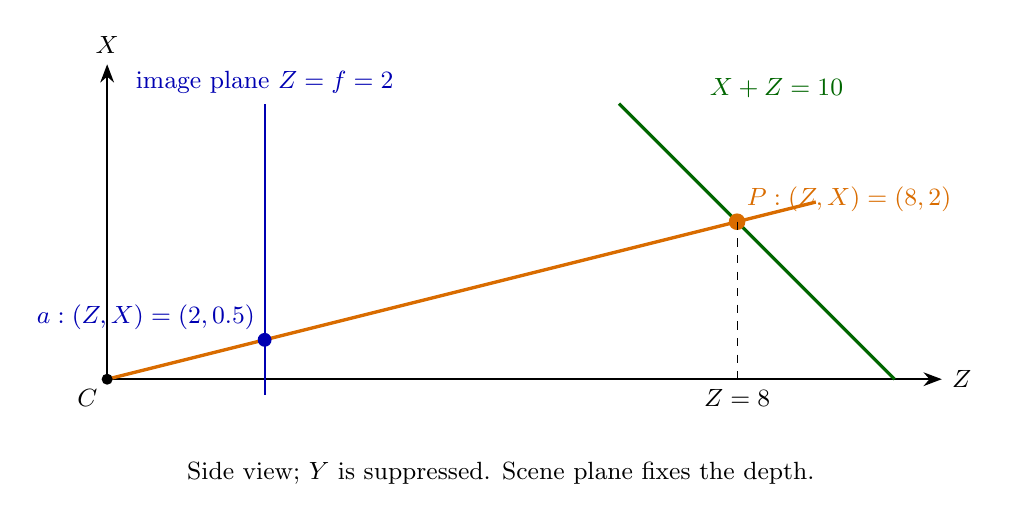
\begin{tikzpicture}[font=\small,arr/.style={-{Stealth},thick},box/.style={draw=blue!55!black,rounded corners,fill=blue!4,align=center,text width=2.9cm,minimum height=1.05cm}]

\draw[arr] (0,0)--(10.6,0) node[right]{$Z$};
\draw[arr] (0,0)--(0,4) node[above]{$X$};
\draw[blue!70!black,thick] (2,-.2)--(2,3.5) node[above]{image plane $Z=f=2$};
\draw[orange!85!black,very thick] (0,0)--(9,2.25);
\draw[green!40!black,very thick] (6.5,3.5)--(10,0);
\node[green!40!black] at (8.5,3.7){$X+Z=10$};
\fill (0,0) circle(2pt) node[below left]{$C$};
\fill[blue!70!black] (2,.5) circle(2.5pt) node[above left]{$a:(Z,X)=(2,0.5)$};
\fill[orange!85!black] (8,2) circle(3pt) node[above right]{$P:(Z,X)=(8,2)$};
\draw[dashed] (8,2)--(8,0) node[below]{$Z=8$};
\node at (5,-1.2){Side view; $Y$ is suppressed. Scene plane fixes the depth.};

\end{tikzpicture}
\end{document}
